\documentclass[conference]{IEEEtran}
% \IEEEoverridecommandlockouts

\usepackage{cite}
\usepackage{amsmath,amssymb,amsfonts}
\usepackage{algorithmic}
\usepackage{graphicx}
\usepackage{textcomp}
\usepackage{xcolor}
\usepackage{tabularx}
\usepackage{array}
\usepackage{subcaption}
\usepackage{booktabs}
\usepackage{multirow}
\usepackage{hyperref}

\newcolumntype{Y}{>{\raggedright\arraybackslash}X}
\newcolumntype{C}{>{\centering\arraybackslash}X}

\def\BibTeX{{\rm B\kern-.05em{\sc i\kern-.025em b}\kern-.08em
    T\kern-.1667em\lower.7ex\hbox{E}\kern-.125emX}}
\begin{document}

\begin{titlepage}
    \centering

    {\Huge\bfseries Extract, then decide: a modular pipeline of LLMs and rules to identify seizure frequency in epilepsy clinic letters \par}
    \vspace{5cm}

    {\large
    A dissertation submitted in partial fulfilment of\par
    The requirement for the degree of\par
    MASTER OF SCIENCE in Artificial Intelligence\par
    in\par
    \par
    The Queen’s University of Belfast\par
    by\par
    Conor Brown\par
    4th September 2026
    }
\end{titlepage}

\onecolumn
\thispagestyle{empty}

\begin{center}
{\Large\bfseries Declaration of Academic Integrity}
\end{center}

\vspace{8pt}

\noindent
I certify that the submission is my own work, all sources are
correctly attributed, and the contribution of any AI technologies
is fully acknowledged.

\vspace{6pt}

\noindent
I declare that I have read both the University and the School of
Electronics, Electrical Engineering and Computer Science guidelines
on plagiarism --
\url{https://www.qub.ac.uk/directorates/sgc/learning/LearningResources/Plagiarism/}
-- and that the attached submission is my own original work. No part
of it has been submitted for any other assignment and I have
acknowledged in my notes and bibliography all written and electronic
sources used.

\vspace{6pt}

\noindent
I am aware of the disciplinary consequences of failing to abide and
follow the School and Queen's University Regulations on Plagiarism.

\vspace{18pt}

\noindent
Name : CONOR BROWN

\vspace{14pt}

\noindent
Student Number: 40466218


\noindent
Student's signature:

\includegraphics[height=2.2cm]{signature.png}
\hfill
Date of submission: 4th September 2026

\clearpage
\twocolumn

\title{Extract, then decide: a modular pipeline of LLMs and rules to identify seizure frequency in epilepsy clinic letters\\}

\maketitle

\begin{abstract}
Seizure frequency is written in clinic letters, and extracting 
it for research still relies on slow, error-prone manual chart 
review. Large language models (LLMs) can read these letters, but 
the best reported result required fine-tuning on over a thousand 
labelled letters. This paper splits the task in two: an LLM 
\texttt{extract}s every candidate frequency with its evidence, 
then a fixed policy \texttt{decide}s the answer. The policy was 
applied by rules (\texttt{Hybrid}) and by a second LLM call 
(\texttt{LLM-only}). Both were evaluated on 1,200 synthetic 
epilepsy letters against the benchmark reported for the 
fine-tuned LLM on a different held-out sample of the same corpus. 
\texttt{Hybrid} (F1 0.86) and \texttt{LLM-only} (0.85) exceeded 
the reported benchmark (0.81) and improved on the extraction 
stage's answer alone (0.79); removing the extraction prompt's 
examples, closed label forms or evidence obligation lowered the 
result. On this synthetic benchmark, a prompted model with a 
separate decision step matched a fine-tuned one.

\end{abstract}

\begin{IEEEkeywords}
information extraction, hybrid pipeline, large language models, seizure frequency, epilepsy
\end{IEEEkeywords}

\section{Introduction}

Epilepsy affects approximately 1\% of the UK population \cite{b1} 
and is characterised by recurrent, unprovoked seizures \cite{b2}. Seizure frequency 
is the primary indicator of disease burden, serving as the central metric guiding 
clinical treatment and the primary endpoint in clinical trials. 
Despite its clinical importance, seizure frequency is rarely recorded in structured 
electronic health record fields; instead, it remains embedded within unstructured 
clinic letters. These narrative documents summarise outpatient consultations, combining 
past medical history, interval symptom changes, and future management plans. Extracting 
this information at scale for retrospective research or cohort identification 
traditionally requires manual chart review, which is labour-intensive, costly, 
and difficult to standardise across institutions.

Natural language processing (NLP) offers an automated alternative, yet clinical 
narrative presents distinct challenges. Traditional rule-based systems provide 
deterministic, auditable logic valued by clinicians, but they struggle with the 
lexical variety and syntactic complexity of clinical frequency descriptions, which 
range from explicit rates (\emph{2 to 3 seizures a week}) to relative interval counts 
(\emph{4 since her last visit}) and qualitative impressions (\emph{frequent bouts}) \cite{b3}. 
Conversely, large language models (LLMs) demonstrate remarkable semantic flexibility 
in zero- and few-shot clinical information extraction \cite{b11, b12}. However, unconstrained 
LLMs introduce substantial clinical risks: they operate as black boxes, remain prone to 
hallucinations or ungrounded assertions \cite{b5}, and existing state-of-the-art results 
have relied on fine-tuning on large collections of expert-annotated letters \cite{b3}.

There is often more than one valid description of a patient's seizure frequency pattern. Clinic letters frequently 
document multiple temporal intervals or distinct seizure types, such as historical baseline 
rates alongside recent breakthrough seizures following an anti-seizure medication titration. 
Selecting which mention reflects the patient's current seizure frequency is a matter 
of clinical policy. When an LLM is asked to produce a single answer to a complex question,
much of the nuance is lost. This prevents clinicians from inspecting the evidence chain 
or reconfiguring the selection criteria for different clinical studies.

To address these limitations, this paper investigates a modular, two-stage architecture that 
decouples evidence extraction from clinical decision-making:
\begin{enumerate}
    \item \texttt{Extract}: An LLM identifies all candidate seizure frequency mentions within the letter, extracting canonical forms alongside verbatim textual evidence.
    \item \texttt{Decide}: An explicit clinical selection policy evaluates the candidate records to determine the primary current frequency pattern.
\end{enumerate}
The decision stage operates over structured extraction records rather than raw text, so it can 
be executed either deterministically via recorded expert rules (\texttt{Hybrid}) or probabilistically 
via a second LLM call (\texttt{LLM-only}).

\subsection{Research Aim, Hypotheses, and Contributions}

The primary aim of this paper is to determine whether a modular pipeline separating 
evidence extraction from clinical policy decisions can match the performance of
fine-tuned models without requiring expensive labelled training data. We investigate three core 
hypotheses:
\begin{itemize}
    \item \textbf{H1 (Decoupling Lift):} Explicitly decoupling candidate mention extraction from policy-based decision improves extraction accuracy over an end-to-end, single-pass LLM prompt.
    \item \textbf{H2 (Executor Equivalence):} A deterministic rule-based decision step applied to structured LLM extraction records performs competitively with a second LLM reasoning step, while offering full auditability.
    \item \textbf{H3 (Training-Free Parity):} In-context few-shot extraction paired with structured evidence obligations can reach parity with published fine-tuned benchmarks on the same corpus.
\end{itemize}

The main contributions of this work are: (1) a transparent, modular information extraction architecture 
separating extraction and decision; (2) an empirical comparison between deterministic rule-based and 
LLM-based decision executors; (3) an ablation study identifying the critical components of the extraction 
prompt (examples, closed label forms, and evidence obligations); and (4) an evaluation across six LLMs 
assessing performance on consumer-grade hardware.

\subsection{Scope and Paper Organisation}

The study is focused on the extraction of current seizure frequency patterns from the 
1,200 synthetic epilepsy clinic letters released by Gan \emph{et al.} \cite{b3}. The use of synthetic 
data provides a controlled, reproducible benchmark with expert gold annotations while avoiding patient 
privacy constraints; however, validation on real-world, multi-centre electronic health records remains 
a defined limitation and subject for future work.

The remainder of this paper is organised as follows. Section~\ref{sec:literature} reviews previous 
approaches to seizure frequency extraction and conceptual framings of clinical IE. Section~\ref{sec:methods} 
details the dataset, pipeline architecture, and evaluation framework. Section~\ref{sec:results} presents 
the empirical results, including benchmark comparisons, ablation studies, and model portability checks. 
Section~\ref{sec:discussion} interprets the findings, discusses clinical implications, and addresses ethical 
considerations and limitations. Finally, Section~\ref{sec:conclusion} concludes and outlines directions for 
future research.

\section{Literature Review}
\label{sec:literature}

Extracting clinical outcomes from outpatient epilepsy narratives has progressed across three paradigms: expert-crafted rule-based systems, fine-tuned transformer representations, and large language models (LLMs). Early pipelines relied on pattern matching and regular expressions \cite{b4, b6, b15, b16}. While rules provide deterministic auditability, they struggle with the lexical diversity of frequency descriptions (\emph{2 to 3 a week}, \emph{frequent bouts}, \emph{4 since her last visit}) and frequently fail to generalise across healthcare institutions \cite{b6, b10}. Subsequent approaches applied clinical BERT models to improve semantic coverage \cite{b7, b9, b10}, using downstream rules solely to normalise dates and counts into standardised units. However, these discriminative models remained bounded by token-classification spans and required extensive task-specific annotated training data.

The emergence of autoregressive LLMs significantly advanced clinical information extraction (IE) \cite{b11, b12}. Zero-shot models can interpret varied clinical phrasing \cite{b8}, but risk generating ungrounded hallucinations or irrelevant advice \cite{b5}. To achieve benchmark reliability, recent studies have relied on supervised fine-tuning; notably, Gan \emph{et al.} \cite{b3} established a state-of-the-art benchmark (micro-F1 0.81) by fine-tuning an LLM on over 1,000 expert-annotated letters. However, fine-tuning imposes heavy operational costs: curating thousands of clinical annotations is expensive, model updates require significant compute, and black-box weights obscure the model's decision logic \cite{b14, b18}.

A fundamental limitation in existing LLM extractors is the conflation of extraction and clinical policy. Clinical IE is conventionally framed as mention detection followed by concept normalisation \cite{b13, b14, b21}. In outpatient narratives, however, a clinic letter frequently documents multiple conflicting mentions, such as historical baselines, distinct seizure types, or post-medication interval changes. Selecting which mention represents the patient's current operational status is a matter of clinical policy. Standard pipelines task an LLM with predicting a single final label in one pass, burying candidate selection inside an uninterpretable inference step. In contrast, concept normalisation in wider biomedical informatics routinely separates candidate generation from candidate ranking \cite{b21}.

This paper addresses the gap between brittle rule-based systems and opaque, fine-tuned LLMs. While prior work restricted rules to lexical parsing or post-processing format repair \cite{b5}, we investigate whether an in-context prompted LLM can generate rich, evidence-grounded candidate records that are then resolved by an explicit decision policy. By evaluating both a deterministic rule-based executor (\texttt{Hybrid}) and a second LLM reasoning step (\texttt{LLM-only}), we test whether a modular, training-free architecture can match the fine-tuned benchmark while preserving an auditable evidence chain from source text to final label.

\section{Methods}
\subsection{Data}
\label{sec:data}

The dataset is a collection of epilepsy clinic letters which 
record a UK patient's consultation with an epilepsy 
specialist, often a neurologist or specialist nurse \cite{b3} 
The NHS requires that clinic letters are sent to the 
patient's GP after all outpatient visits such as these.
They are often the only record of a patient's diagnoses,
treatments and outcomes in neurological disorders, 
and they are written in narrative form. An example clinic letter 
is shown in Figure~\ref{letter}.

\begin{figure}[t]
    \centering

    
\includegraphics[width=\linewidth]{example_clinic_letter.png}
    \caption{An example clinic letter with two distinct seizure frequency patterns highlighted as potential candidates.}
    \label{letter}
\end{figure}

Gan \emph{et al.}\cite{b3}  produced this dataset of synthetic 
letters modelled on real clinic letters from King's College 
London hospital. The real letters were used to create 10 
template letters and they were combined with 500 short 
descriptions of seizure frequency patterns produced 
by GPT-5 to create the full set of 15,099 letters. A sample 
of 1,200 letters of c. 400 words was used in this paper. 
Trained experts annotated each letter with a single 
gold-standard label representing the patient's current seizure 
frequency status, and with one supporting quote.

\begin{table}[!t]
\caption{Dataset summary}
\label{tab:dataset}
\centering
\begin{tabularx}{\linewidth}{lYcc}
\toprule
 & & \textbf{Development} & \textbf{Test} \\
\midrule
\multicolumn{2}{l}{Number of letters} & 750 & 450 \\
\midrule
\multirow{4}{*}{Seizure frequency} & Frequent & 51\% & 50\% \\
 & Infrequent & 17\% & 18\% \\
 & Unknown & 17\% & 17\% \\
 & Seizure free & 15\% & 15\% \\
\bottomrule
\end{tabularx}
\end{table}

Minimal preprocessing was applied: letters were cleaned only 
to parse quotes, new lines, tabs, the $\leq$ sign and nulls, 
and were ingested in full with no tokenisation, 
section-splitting or truncation.

The dataset was split into a development set of 750
letters and a test set of 450 letters, stratified by their 
seizure frequency category (frequent, infrequent, 
unknown, seizure free) to balance the distribution 
across both splits. The exact breakdown can be 
seen in Table~\ref{tab:dataset}.

\subsection{Architecture}

The pipeline has two stages: \texttt{extract}, then 
\texttt{decide}. \texttt{Extract} is one LLM call that reads 
the full letter and returns a structured record of every 
candidate seizure frequency event, each with its exact quoted 
evidence span, a category and a label in one of the canonical 
forms used by the gold standard. The same call also proposes a 
provisional answer from its own candidates. Scoring that answer 
gives a baseline for a single prompt; the \texttt{decide} stage then confirms 
or replaces it. \texttt{Decide} receives that record, not the 
letter, and produces the final answer by applying a fixed 
decision policy, either picking one candidate or combining 
several. Figure~\ref{pipeline} illustrates the pipeline with a 
development-set example.

The decision was performed in two ways on the same 
extraction record (Table~\ref{tab:method}). In \texttt{Hybrid}, 
rules apply the policy. In \texttt{LLM-only}, a second 
LLM call applies the same policy, expressed as written 
instructions and worked examples. The only difference between 
the two is therefore who performs \texttt{decide}; the 
extraction call, its output and the policy are shared. Because 
\texttt{decide} works from that record, both executors 
were replayed on the same extraction output without a new 
model call, so any difference between them is attributable to 
who performed \texttt{decide}.

The pipeline is a fixed sequence of calls and functions. Each LLM 
call is a prompt with a fixed input and a schema-validated JSON 
output. A rules-only baseline and several further 
decompositions of the LLM work were also built and are 
described in the supporting materials; they are not part of 
the main comparison.

\begin{figure*}[t]
    \centering

    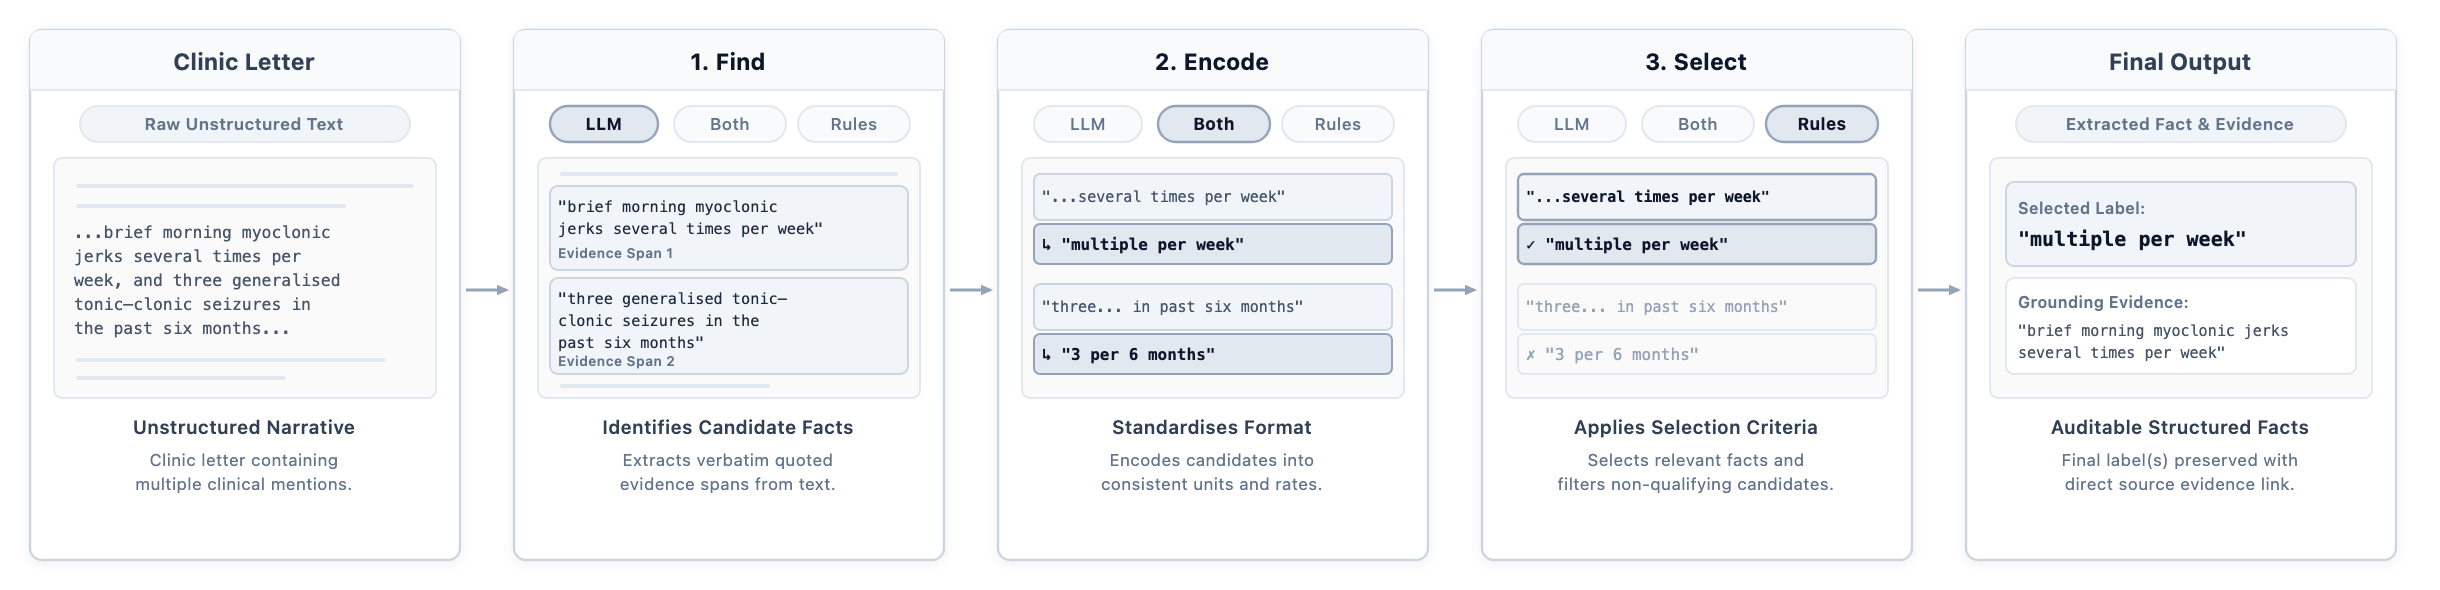
\includegraphics[width=\linewidth]{pipeline_architecture.png}
    \caption{A clinic letter is processed by \texttt{extract}, then \texttt{decide}, to produce a structured label with grounding evidence. \texttt{Extract} is one LLM call. \texttt{Decide} works from the resulting record and is performed by rules (\texttt{Hybrid}) or by a second LLM call (\texttt{LLM-only}).}
    \label{pipeline}
\end{figure*}

\begin{table}[!t]
\caption{What each stage receives and returns}
\label{tab:method}
\centering
\begin{tabularx}{\linewidth}{lYY}
\toprule
 & \textbf{Extract} & \textbf{Decide} \\
\midrule
Input & Full letter & Candidate record and decision policy; not the letter \\
Output & Candidate record: events, each with quoted span, category and canonical label; provisional answer & Final label and its supporting event(s) \\
Performed by & LLM call 1 & \texttt{Hybrid}: rules. \texttt{LLM-only}: LLM call 2 \\
\bottomrule
\end{tabularx}

\vspace*{2pt}
\begin{minipage}{\linewidth}
\raggedright\footnotesize
\texttt{Hybrid} and \texttt{LLM-only} share the first call and the extraction record. Full prompts and schemas are in the supporting materials.
\end{minipage}
\end{table}

\subsection{LLM Prompt Design}

The most consequential component of the pipeline is the 
\texttt{extract} prompt used for the first call. It has four 
ingredients, each of which is removed in turn in 
Section~\ref{sec:ablations}:

\begin{enumerate}
\item \emph{Instructions} to identify relevant seizure frequency 
events and to propose a provisional answer.
\item \emph{Examples} of how events should be represented.
\item \emph{Allowed labels}: a closed list of the canonical 
label forms used by the gold standard.
\item An \emph{evidence obligation}: schema fields for the 
evidence span of every event, with the instruction that each 
span must be an exact quote from the letter.
\end{enumerate}

The output schema represents multiple seizure frequency 
patterns with exact evidence, so that rules or a second LLM 
call can work from the candidates rather than from the letter. 
The same decision policy (Table~\ref{tab:policy}) is applied 
twice: provisionally by the model inside the extraction prompt, 
and finally at \texttt{decide}. For example, if the model finds 
\emph{3 seizures in March, 6 in May} and provisionally answers 
with the most recent count, the \texttt{decide} stage can 
replace that with the total over the whole period, \texttt{9 
per 3 months}, using the evidence the model already found. The 
second-call \texttt{decide} prompt states the same policy as 
written instructions with worked examples and receives only the 
candidate record.

\begin{table}[!t]
\caption{Decision policy}
\label{tab:policy}
\centering
\begin{tabularx}{\linewidth}{YY}
\toprule
\textbf{When} & \textbf{Do} \\
\midrule
Several current seizure types are present &
Choose the highest current or recent frequency. \\
The letter gives an overall current count and a
breakdown by type &
Choose the overall count. \\
A seizure-free statement sits with other current
seizure-like events &
Keep seizure-free separate from unknown or last-event
statements. \\
\bottomrule
\end{tabularx}
\end{table}

The model is instructed to assign each event to one of six 
categories (a countable or range \emph{frequency rate}, a 
\emph{cluster frequency}, a \emph{seizure-free} statement, a 
dated \emph{last event} without a rate, an \emph{unknown 
frequency} where seizures are discussed without a usable rate, 
and \emph{no reference}) and to write its label in one of the 
canonical forms listed in the prompt. The category definitions, 
label forms and full prompt are in the supporting materials.

\subsection{Rule Design}

In \texttt{Hybrid}, rules perform \texttt{decide}. 
Each rule is a named function with \texttt{regex} matching and 
if-then logic that reads the candidate record the model 
returned, not the letter. Rules first rewrite any label the 
model left in a non-canonical form (a step that changes the 
score by at most 0.01 and is detailed in the supporting 
materials), then apply the decision policy in 
Table~\ref{tab:policy}. Three kinds of decision rule are used. 
A \emph{gate} rejects a provisional answer that the policy 
forbids: if the model finds both \emph{seizure free for eight 
months} and \emph{two seizures in the past fortnight} but 
provisionally answers seizure-free, the gate rejects 
seizure-free while other current seizure-like events remain. A 
\emph{reselect} rule chooses a different already-extracted 
event, such as a frequency candidate when the model chose 
\texttt{unknown}. A \emph{rewrite} rule derives a new label from 
the extracted events: for seizure diaries, date and numeric 
logic totals the events over the stated period, so \emph{May 
x0, Jun x0, Jul x1, Aug x0, Sep x1, Oct x2} becomes \texttt{4 
per 6 months}. Every rule is recorded with the event it acted 
on, so a final label can be traced to the model's quoted 
evidence and the rule that decided it. Rules do not scan the 
letter for new candidates; every rule acts on the events the 
model extracted.

\subsection{Pipeline Optimisation}

The development set was used to optimise the two key 
elements of the pipeline: the LLM prompt instructions and 
the rules. The focus of the optimisation process was to 
improve accuracy while keeping the instructions and rules 
simple and generalisable. Qualitative error analysis was 
conducted to diagnose the cause of poor performance and 
identify common error modes. Hypotheses were developed 
and tested to tune the prompt and rules iteratively. 
Improving a rule or instruction for one class of error 
often harmed another, because the annotation policies 
interact. Separating \texttt{extract} from \texttt{decide} 
kept the policy on which facts to extract apart from the 
policy on which to choose, and made it possible to score the 
pipeline after each stage and locate bottlenecks. The 
supporting materials give a fuller account of this process.

\subsection{Evaluation}
\label{sec:evaluation}

Every paper reporting seizure frequency extraction this 
decade used F1 as its primary metric, but they differ in 
what counts as a correct frequency label. It is not obvious 
whether \emph{2 per month}, \emph{3 per month} and 
\emph{once a week} should all be accepted when the 
gold-standard label is \emph{multiple per month}. To allow 
comparison with Gan \emph{et al.}\cite{b3}, this paper adopts 
their two evaluation settings: a fine-grained \texttt{purist} 
setting and a coarser \texttt{pragmatic} setting. If the gold 
label is \emph{twice a week} and the prediction is \emph{once 
a week}, that is a correct \texttt{pragmatic} answer, since 
both fall in the \texttt{frequent} category, but an incorrect 
\texttt{purist} answer. Table~\ref{tab:performance} lists the 
categories in each setting.

Micro-F1 is reported for both settings, because the 
categories are badly imbalanced (some have over 100 letters, 
some fewer than 10; Table~\ref{tab:performance}) and micro-F1 
gives each letter equal weight. Each letter has exactly one 
gold label and one prediction, so micro-F1 here equals the 
share of letters answered correctly. The more precise 
\texttt{purist} F1 is the primary metric.

The pipeline is evaluated on a held-out test set of 450 
letters that were never used to tune prompts, rules or any 
other aspect of the pipeline. Results are compared against 
the evaluation set labelled Synthetic (1,166) in Gan 
\emph{et al.}\cite{b3}, a different held-out sample from the 
same synthetic corpus, distinct from their fine-tuning data.

The primary model is Gemini 3.7 Flash. It is the only model 
used for the second decision call (\texttt{LLM-only}), for the 
prompt ablations and for the temperature and thinking-level 
ablations. Six models were evaluated as the extraction call in 
\texttt{Hybrid} (Section~\ref{sec:models}). Elsewhere, 
\texttt{Hybrid} results are from Gemini at temperature 0 with 
low thinking effort. The held-out results are reported as 
aggregate totals only; individual test letters and their 
outputs were not inspected.

\section{Results}

\subsection{Benchmark Performance}
\label{sec:benchmark}

The primary objective of this paper is to evaluate whether 
a prompted LLM and rules can match 
a fine-tuned LLM at extracting seizure frequency patterns from 
epilepsy letters. Results are compared with the Synthetic 
(1,166) evaluation reported by Gan \emph{et al.}\cite{b3}. The 
two evaluations use identical metric definitions and letters 
drawn from the same synthetic corpus, but different held-out 
samples. The comparison is therefore with a previously reported 
benchmark, not a paired evaluation on the same letters, and it 
does not establish a state-of-the-art result.

\texttt{Hybrid} achieves a \texttt{purist} F1 of 0.86 
(387/450), above the reported benchmark of 0.81 for the 
fine-tuned LLM. \texttt{LLM-only} also exceeds it (0.85; 
383/450). Because micro-F1 equals per-letter accuracy here, 
an approximate two-proportion comparison gives a difference 
of +0.05 for \texttt{Hybrid} (95\% CI +0.01 to +0.09, 
$p = 0.01$) and +0.04 for \texttt{LLM-only} (95\% CI 0.00 to 
+0.08, $p = 0.04$). These intervals assume independent samples 
from the same distribution and are indicative rather than a 
controlled comparison. The first LLM call alone, scored on its 
provisional answer, reaches 0.79, close to the benchmark. 
Rules applied to its candidates add +0.07 in \texttt{Hybrid}; 
the second LLM call adds +0.06 in \texttt{LLM-only}.

The pipeline is particularly effective at extracting 
high-frequency events. Gan \emph{et al.} report \texttt{unknown} 
as their highest scoring category (0.89), with \texttt{daily} (0.70) 
and \texttt{more than weekly} (0.68) much lower. In this pipeline, 
\texttt{daily} (0.92) and \texttt{more than weekly} (0.91) are among the 
best performing categories, well above \texttt{unknown} (0.74). 
The full breakdown across \texttt{purist} and \texttt{pragmatic} 
categories is in Table~\ref{tab:performance}.

\begin{table}[!t]
\caption{Comparison with previously reported results}
\label{tab:historical}
\centering
\begin{tabularx}{\linewidth}{Yclll}
\toprule
\textbf{Author} & \textbf{Year} & \textbf{Method} & \textbf{Purist F1} & \textbf{Pragmatic} \\
\midrule
Holgate et al. & 2024 & Prompted LLM & - & 0.73 \\
Holgate et al. & 2025 & Fine-tuned LLM & 0.68 & 0.81 \\
Gan et al. & 2026 & Fine-tuned LLM & 0.81 & 0.85 \\
\midrule
This paper & 2026 & Hybrid (LLM + rules) & 0.86 & 0.88 \\
\bottomrule
\end{tabularx}

\vspace*{2pt}
\begin{minipage}{\linewidth}
\raggedright\footnotesize
Each row was evaluated on a different held-out sample; only Gan et al. and this paper share a corpus and metric definitions.
\end{minipage}
\end{table}

\begin{table}[!t]
\caption{Hybrid: Purist and Pragmatic categories (test set, $n = 450$)}
\label{tab:performance}
\centering
\begin{tabularx}{\linewidth}{Yccc}
\toprule
\textbf{Purist} &
\textbf{\emph{n}} &
\textbf{Purist F1} &
\textbf{Pragmatic F1} \\
\midrule
Daily & 41 & 0.92 & \multirow{4}{*}{Frequent: 0.95} \\
More than weekly, less than daily & 123 & 0.91 & \\
Once a week & 5 & \textcolor{black!55}{0.89} & \\
More than monthly, less than weekly & 58 & 0.90 & \\
\midrule
Once a month & 18 & 0.94 & \multirow{4}{*}{Infrequent: 0.82} \\
More than every 6 months, less than monthly & 55 & 0.81 & \\
Once every 6 months & 1 & \textcolor{black!55}{0.00} & \\
Less than once every 6 months & 6 & \textcolor{black!55}{0.60} & \\
\midrule
Unknown & 76 & 0.74 & Unknown: 0.74 \\
\midrule
Seizure free & 67 & 0.90 & Seizure free: 0.90 \\
\bottomrule
\end{tabularx}

\vspace*{2pt}
\begin{minipage}{\linewidth}
\raggedright\footnotesize
Rows with $n{<}10$ shown in grey.
\end{minipage}
\end{table}

\subsection{Provisional and Final Answers}
\label{sec:stages}

Table~\ref{tab:stages} reports \texttt{purist} F1 at two 
stops: the provisional answer after \texttt{extract}, and the 
final answer after \texttt{decide}, for each decision executor. 
Each stop scores the answer the pipeline would submit if it 
stopped there. The provisional answer is the extraction call's 
own proposal, so its score measures the quality of that 
proposal, not candidate identification alone. The difference 
between the columns is what \texttt{decide} adds to the answer 
already proposed.

The provisional answer from the single extraction call is 0.79. 
This call is equivalent to the entire pipeline in most prior 
LLM studies, which ask the model to extract and decide in one 
prompt. Both executors then improve on that shared provisional 
answer at \texttt{decide}: rules add +0.07 and the second LLM 
call adds +0.06. This can mean choosing a different candidate, 
such as a frequency candidate when the model chose 
\texttt{unknown}, or calculating a new label from the chosen 
evidence, such as totalling the events in a monthly seizure 
diary. The two executors differ on 28 of 450 letters (rules 
correct on 16, the second call on 12); a paired McNemar test 
gives a difference of +0.01 (95\% CI $-$0.01 to +0.03, 
$p = 0.57$), compatible with no difference. Applying the 
decision policy to the candidates already extracted is where 
the pipeline adds value over a single prompt, and on this task 
it can be performed as well by rules as by a second 
LLM call. Other decompositions of the LLM work, including a 
separate label-rewriting call before \texttt{decide}, did not 
improve on this design and are reported in the 
supporting materials.

\begin{table}[!t]
\caption{Purist F1 after each stage, by decision executor}
\label{tab:stages}
\centering
\begin{tabularx}{\linewidth}{lCC}
\toprule
\textbf{Decision executor} &
\textbf{Provisional answer (after extract)} &
\textbf{Final answer (after decide)} \\
\midrule
Hybrid: rules & 0.79 (355) & 0.86 (387) \\
LLM-only: second LLM call & 0.79 (355) & 0.85 (383) \\
\bottomrule
\end{tabularx}

\vspace*{2pt}
\begin{minipage}{\linewidth}
\raggedright\footnotesize
Correct letters of 450 in parentheses. Both rows share the same extraction call and record; only \texttt{decide} differs.\end{minipage}
\end{table}

\subsection{Extraction Prompt Ablations}
\label{sec:ablations}

Table~\ref{tab:ablations} removes one ingredient of the 
extraction prompt at a time and scores the \texttt{Hybrid} 
pipeline at both stops, so the effect of each ingredient can be 
seen on the provisional answer and after rules have applied the 
policy. Removing the worked examples, the closed list of allowed 
label forms, or the evidence obligation each lowers the 
provisional answer by 8 to 10 letters and the final answer by 
17 to 23 letters. The evidence-obligation ablation removes the 
evidence fields and the exact-quote instruction together as one 
package; it does not test the quote instruction alone. The 
decrements are not additive and should not be summed: each row 
removes one ingredient from the full prompt while the others 
remain. Rules recover some of each loss but never the whole of 
it, which shows that the decision stage depends on the quality 
of the record the extraction call produces.

\begin{table}[!t]
\caption{Extraction prompt ablations (Hybrid, Gemini, test set)}
\label{tab:ablations}
\centering
\begin{tabularx}{\linewidth}{YCC}
\toprule
\textbf{Extraction prompt} &
\textbf{Provisional answer} &
\textbf{Final answer} \\
\midrule
Full prompt & 0.79 (355) & \textbf{0.86} (387) \\
Without examples & 0.77 (345) & 0.82 (370) \\
Without closed allowed-label forms & 0.77 (347) & 0.81 (364) \\
Without evidence obligation & 0.77 (345) & 0.82 (370) \\
\bottomrule
\end{tabularx}

\vspace*{2pt}
\begin{minipage}{\linewidth}
\raggedright\footnotesize
Purist F1 with correct letters of 450 in parentheses. Each row changes only the extraction prompt; the same rules apply the policy at \texttt{decide}. Effects are not additive.\end{minipage}
\end{table}

\subsection{Model Comparison}
\label{sec:models}

\texttt{Hybrid} shows consistent, incremental gains on each 
of the six models evaluated as the extraction call 
(Figure~\ref{models}). The average gain from the provisional 
answer to the final answer was +0.07, with Luna showing the 
largest gain of +0.10. \texttt{Purist} F1 closely tracks 
general medical capability as measured by Artificial Analysis' 
Healthcare and Medical Index. The models cluster into three 
groups: strong (Gemini 0.86, Grok 0.85), medium (DeepSeek 
0.82, Luna 0.79) and weak (Qwen 0.76, Gemma 0.72), which 
largely reflect model size and cost.

Table~\ref{tab:adherence} reports how well each model kept to 
the extraction contract. Every model produced a parseable 
record for at least 442 of 450 letters, and no call failed. 
The four hosted models quoted an exact substring of the letter 
as evidence for the selected event in 99\% or more of letters; 
the two local models paraphrased more often (Qwen 97\%, Gemma 
93\%) and needed more non-semantic format repair. An exact span 
is not proof that the right statement was chosen, but it means 
that a reviewer can locate the evidence for almost every answer 
verbatim in the source.

Table~\ref{tab:historical} also lists the two earlier papers 
that used the same \texttt{pragmatic} metric on different 
data. Holgate \emph{et al.}\cite{b8} ran Llama 2 on local 
hospital servers with eight Nvidia V100 GPUs and reached a 
\texttt{pragmatic} F1 of 0.73 without fine-tuning. In 
\texttt{Hybrid}, Qwen reached a \texttt{pragmatic} F1 of 0.80 
running locally on a laptop with a single GPU. This shows that 
the design can execute on local 
hardware under the same synthetic task conditions, not that it 
performs on real letters or is fit for deployment.

\begin{figure}[t]
    \centering

    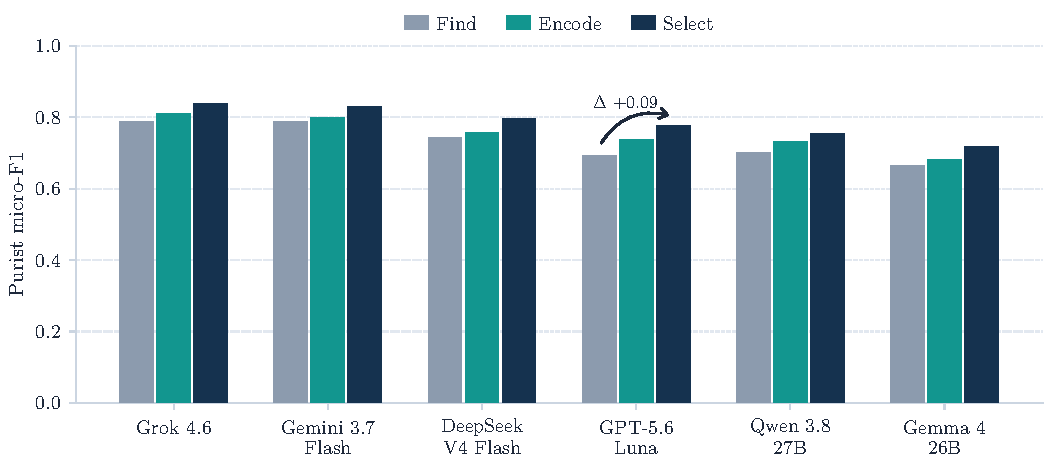
\includegraphics[width=\linewidth]{six_model_stage_performance.pdf}
    \caption{\texttt{Hybrid} Purist F1 for six models: the LLM's provisional answer after \texttt{extract} and the final answer after rule-based \texttt{decide}. Every model gains at \texttt{decide}; Luna gains most (0.69 to 0.79).}
    \label{models}
\end{figure}

\begin{table}[!t]
\caption{Six models as the extraction call: scores and contract adherence (Hybrid, test set, $n = 450$)}
\label{tab:adherence}
\centering
\footnotesize
\begin{tabularx}{\linewidth}{Yrrrrr}
\toprule
\textbf{Model} & \textbf{Purist} & \textbf{Prag.} & \textbf{Exact ev.} & \textbf{Repairs} & \textbf{Unparsed} \\
\midrule
Gemini 3.7 Flash & \textbf{0.86} & 0.88 & 99.8\% & 0 & 1 \\
Grok 4.6 & 0.85 & \textbf{0.89} & 100\% & 0 & 0 \\
DeepSeek V4 Flash & 0.82 & 0.85 & 99.6\% & 2 & 0 \\
GPT-5.6 Luna & 0.79 & 0.82 & 98.9\% & 0 & 1 \\
Qwen 3.8 27B (local) & 0.76 & 0.81 & 96.7\% & 3 & 2 \\
Gemma 4 26B (local) & 0.72 & 0.77 & 92.9\% & 15 & 8 \\
\bottomrule
\end{tabularx}

\vspace*{2pt}
\begin{minipage}{\linewidth}
\raggedright\footnotesize
Exact ev.: the quoted span for the selected event is an exact substring of the letter. Repairs: letters needing a non-semantic JSON dialect repair. Unparsed: letters with no valid record after repair, scored as incorrect. No call failed for any model.\end{minipage}
\end{table}

\subsection{Model Configuration}

Raising the reasoning effort level did not improve 
performance. Gemini's \texttt{purist}-F1 score was 0.86 at low and 
0.84 at high; a paired difference of +0.02, 95\% CI -0.01 to 
0.04; p = 0.31. Extra reasoning adds cost and latency without 
improving extraction.

The temperature setting also had no significant effect: 0.86 
at temperature 0 versus 0.84 at temperature 1 (paired 
difference +0.02, 95\% CI -0.01 to 0.04; p = 0.20). Temperature 
0 is therefore an appropriate default, and Luna's fixed 
temperature of 1 does not invalidate its comparison. The task 
is tightly defined by an explicit schema, which limits the 
expected variability by design and partly explains why neither 
setting mattered.

\subsection{Error Analysis}
\label{sec:errors}

The worst performing category was \texttt{unknown} with 
an F1 score of 0.74. 69\% of the errors (37/54) are incorrect
answers of \texttt{unknown}. The full error distribution 
is shown in the confusion matrix (Figure~\ref{confusion}). 

The three most common errors are \texttt{infrequent → 
unknown} (16), \texttt{frequent → unknown} (13), and 
\texttt{seizure free → unknown} (8). The errors reflect a 
cautious approach when the evidence is ambiguous,
for example the model recognised the phrase 'these 
episodes crop up most shifts' as the primary seizure 
frequency description but refused to make an 
assumption about how many shifts the person works. The 
gold-standard label was \texttt{multiple per week} but the 
model chose \texttt{unknown}. This cautious assessment 
is justifiable, and because the exact evidence is preserved, 
downstream users can see the proposed answer and draw their 
own conclusion from the quoted span.

\begin{figure}[t]
    \centering

    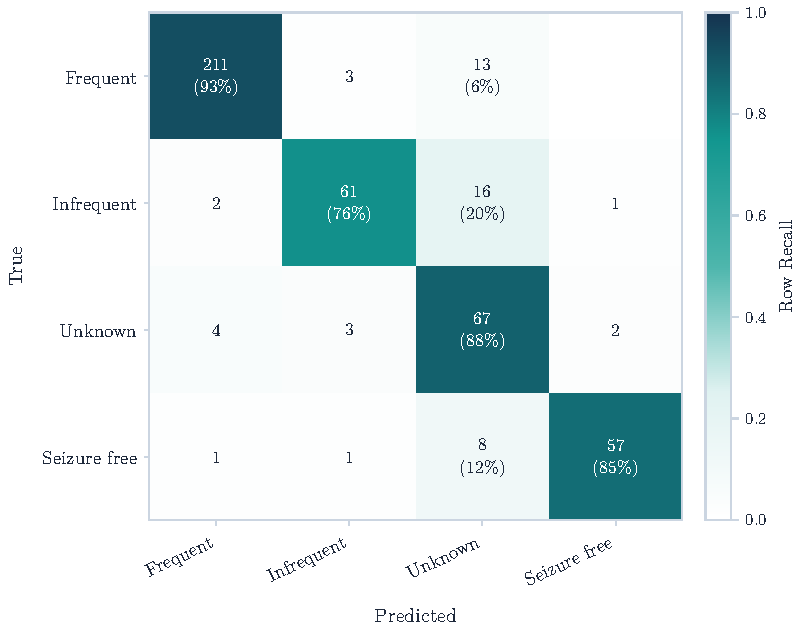
\includegraphics[width=\linewidth]{confusion_matrix_pragmatic.pdf}
     \caption{\texttt{Hybrid} confusion matrix on the \texttt{pragmatic} categories (test set). Most errors are incorrect predictions of \texttt{unknown}.}
    \label{confusion}
\end{figure}

\subsection{Experimental Environment}

Table~\ref{tab:environment} summarises the hardware, software 
and model settings used. DSPy co-ordinated the model calls and 
required structured JSON output, Pydantic validated each record 
against the schema, and LiteLLM delivered API calls to Ollama 
and the model routers. Full specifications, API settings and 
replay artefacts are in the supporting materials.

\begin{table}[!t]
\caption{Experimental environment}
\label{tab:environment}
\centering
\begin{tabularx}{\linewidth}{lY}
\toprule
\textbf{Component} & \textbf{Setting} \\
\midrule
Local models & Qwen 3.8 27B and Gemma 4 26B served by Ollama 0.32.15 on a Dell XPS 16 9640 (Windows 11, Intel Core Ultra 9 185H, 32 GB RAM, NVIDIA RTX 4070 Laptop GPU, 8 GB VRAM) \\
Hosted models & Gemini 3.7 Flash, Grok 4.6, GPT-5.6 Luna and DeepSeek V4 Flash, called from a Mac mini M1 (16 GB, macOS 26.5.2) directly (OpenAI, DeepSeek) or via OpenRouter and AI Gateway \\
Model settings & Temperature 0 (Luna accepts only 1); thinking or effort level low. Gemini ablations: temperature 1; thinking medium and high \\
Software & Python 3.14.4, DSPy 3.2.1, Pydantic 2.13.4, LiteLLM 1.87.1 \\
\bottomrule
\end{tabularx}
\end{table}

\section{Discussion}

This paper shows that, on the Gan synthetic benchmark, one 
prompted LLM call and a 
decision policy extract an epilepsy patient's current seizure 
frequency pattern at least as accurately as the fine-tuned LLM 
previously reported on a different held-out sample of the same 
corpus\cite{b3}. A single prompt designed to extract every 
candidate with exact evidence, followed by rules or a second 
call that decide from that evidence, matched that benchmark. 
The same 
design also executed on a laptop-class GPU with open-weight 
models, at a lower but still competitive score. Later 
researchers or healthcare 
organisations can evaluate it on their own data and hardware; it 
is not ready for local deployment.

The method is particularly effective at identifying the 
categories that mark the greatest disease burden. F1 scores of 
0.92 for daily and 0.91 for more than weekly are around 0.2 
higher than the category scores previously reported\cite{b3}, 
although on a different sample. Structured seizure frequency 
of this kind is intended for later research uses: cohort 
identification for trials, retrospective and longitudinal 
analyses of treatment response, and outcome variables for 
predictive models\cite{b13}, which together can widen the 
scope of real-world evidence\cite{b17}. Those are intended 
uses, not capabilities demonstrated here; each requires 
validation on real records first. 

Past work has typically tasked the LLM with producing a single 
answer in a fully normalised form\cite{b3}. That discards the 
semantic depth of the narrative, which clinicians value because 
it conveys reasoning, uncertainty and vague impressions, and 
those nuanced observations are more accurate and 
reliable\cite{b18}. Current LLMs can populate a richer record 
that preserves them: every candidate with its quoted span, the 
policy applied, and the label it produced. The ablations show 
that this record is also what the accuracy depends on. A more 
explainable system is often a more useful system in a clinical 
setting\cite{b14}, and here it is not a less accurate one.

There are several limitations. Synthetic data was used for 
all evaluations, and while past research has shown models 
fine-tuned on this dataset generalise effectively to real 
patient data\cite{b3}, the methods tested here remain untested 
on real letters; no claim is made about clinical validity, 
workflow fit or privacy compliance. The held-out samples 
differ. Past research has shown that rules tuned on one corpus 
can generalise poorly to others, so the gains from rules may 
not transfer to other datasets\cite{b6}. The stage scores are 
cumulative stops rather than isolated stage metrics. Evidence 
quality was measured only as exact-substring adherence, which 
does not show that a span semantically supports the label; the 
gold standard's single reference quote is a loose comparator 
for that purpose, since it may be paraphrased or abbreviated. A 
development-set study of semantic evidence sufficiency, 
adjudicated from the extracted spans and the policy alone, is 
specified as the next step before any further held-out 
evaluation. Finally, the method was applied to one narrow task. 
The same method has been configured for a multi-fact 
epilepsy inventory task\cite{b4}, to be reported separately, 
and future work should evaluate whether the design generalises 
to other clinical IE tasks and whether a more general 
framework, in which an LLM chooses how to represent facts and 
which policy to apply, adds value as reported in 
oncology\cite{b19} and cardiology\cite{b20}.

\section{AI Ethical Considerations}

This evaluation used only the synthetic clinic letters released
by Gan \emph{et al.}\cite{b3}. Those letters are modelled on real
UK epilepsy letters but do not contain identifiable patient records. 
Hospitals prefer processing patient data on their own servers as
it is highly sensitive\cite{b5}. Two of the six models were 
run entirely on local hardware to test whether the design can 
execute in such a setting on synthetic data, not as a 
privacy-compliance assessment.

LLMs can invent evidence, so careful consideration was given
to the prompt instructions and schema design. The model is
required to quote exact evidence spans from the letter, and 
every later change to the answer is made by a named rule or 
a second call applied to that quoted evidence. A 
reviewer can therefore trace any final label back to the 
text that supports it and to the policy that decided 
it\cite{b14}. This transparency matters more than headline 
accuracy in a clinical setting, where an unexplained answer 
cannot be safely acted on.

The letters contain no demographic attributes, so unequal
performance across patient groups cannot be tested, and the 
synthetic corpus may not reflect the language of every 
clinic. Bias can enter through the models, the prompts and 
the decision rules; for example, the cautious default to 
\texttt{unknown} (Section~\ref{sec:errors}) would 
systematically under-count patients whose seizures are 
described vaguely. Rules make the decision policy 
inspectable and changeable by local clinicians, but they do 
not remove the need for local clinical review and fairness 
testing on real records before any operational use.

\section{Conclusion}

Seizure frequency is a core outcome measure in epilepsy, 
recorded almost exclusively in narrative clinic letters. This 
paper proposes a pipeline in which 
one LLM call extracts every candidate fact with its quoted 
evidence in a canonical form, then a decision applies a 
fixed policy to those candidates. 

Both \texttt{Hybrid} (Purist F1: 0.86) and \texttt{LLM-only} 
(0.85) exceeded the benchmark previously reported for a 
fine-tuned LLM (0.81) on a different held-out sample of the 
same synthetic corpus. The provisional 
answer reaches 0.79; applying the decision policy to the 
evidence it found adds a further +0.06 to +0.07, whether that 
policy is applied by rules or by a second LLM call. 
The result depends on the extraction prompt's examples, closed 
label forms and evidence obligation, and it held across six 
models, including two run on a single laptop GPU.

Automatically extracting seizure frequency patterns from 
electronic health records could make this outcome measure available for large-scale 
clinical research: cohort identification, retrospective 
studies and predictive modelling. Future research should evaluate it on real 
patient data and on a broader set of clinical information 
extraction tasks before any of those uses.

\begin{thebibliography}{00}

\bibitem{b1} S. Wigglesworth, A. Neligan, J.~M. Dickson, A. Pullen, E. Yelland, T. Anjuman, and M. Reuber, ``The incidence and prevalence of epilepsy in the United Kingdom 2013--2018: A retrospective cohort study of UK primary care data,'' \emph{Seizure}, vol.~105, pp.~37--42, 2023.
\bibitem{b2} R.~S. Fisher \emph{et al.}, ``ILAE official report: A practical clinical definition of epilepsy,'' \emph{Epilepsia}, vol.~55, no.~4, pp.~475--482, 2014.
\bibitem{b3} Y. Gan \emph{et al.}, ``Reproducible synthetic clinical letters for seizure frequency information extraction,'' arXiv:2603.11407, 2026.
\bibitem{b4} B. Fonferko-Shadrach \emph{et al.}, ``Annotation of epilepsy clinic letters for natural language processing,'' \emph{J. Biomed. Semantics}, vol.~15, no.~17, 2024.
\bibitem{b5} B. Holgate, J. Davies, S. Fang, J.~S. Winston, J.~T. Teo, and M.~P. Richardson, ``Fine-tuning LLMs to extract epilepsy seizure frequency data from health records,'' in \emph{Proc. 24th Workshop on Biomedical Language Processing (BioNLP)}, 2025, pp.~44--55.
\bibitem{b6} B.~M. Decker \emph{et al.}, ``Development of a natural language processing algorithm to extract seizure types and frequencies from the electronic health record,'' \emph{Seizure}, vol.~101, pp.~48--51, 2022.
\bibitem{b7} K. Xie \emph{et al.}, ``Extracting seizure frequency from epilepsy clinic notes: a machine reading approach to natural language processing,'' \emph{J. Amer. Med. Informat. Assoc.}, vol.~29, no.~5, pp.~873--881, 2022.
\bibitem{b8} B. Holgate, S. Fang, A. Shek, M. McWilliam, P. Viana, J.~S. Winston, J.~T. Teo, and M.~P. Richardson, ``Extracting epilepsy patient data with Llama 2,'' in \emph{Proc. 23rd Workshop on Biomedical Natural Language Processing (BioNLP)}, 2024, pp.~526--535.
\bibitem{b9} K. Xie, B. Litt, D. Roth, and C.~A. Ellis, ``Quantifying clinical outcome measures in patients with epilepsy using the electronic health record,'' in \emph{Proc. BioNLP Workshop}, 2022, pp.~369--375.
\bibitem{b10} M. Fernandes, A. Cardall, L.~M.~V.~R. Moura, C. McGraw, S.~F. Zafar, and M.~B. Westover, ``Extracting seizure control metrics from clinic notes of patients with epilepsy: A natural language processing approach,'' \emph{Epilepsy Res.}, vol.~207, 2024, Art.~no.~107451.
\bibitem{b11} T. Brown \emph{et al.}, ``Language models are few-shot learners,'' in \emph{Adv. Neural Inf. Process. Syst. (NeurIPS)}, vol.~33, 2020, pp.~1877--1901.
\bibitem{b12} M. Agrawal, S. Hegselmann, H. Lang, Y. Kim, and D. Sontag, ``Large language models are few-shot clinical information extractors,'' in \emph{Proc. Conf. Empirical Methods in Natural Language Processing (EMNLP)}, 2022, pp.~1998--2022.
\bibitem{b13} L. Cui, S.~S. Sahoo, S.~D. Lhatoo, G. Garg, P. Rai, A. Bozorgi, and G.-Q. Zhang, ``Complex epilepsy phenotype extraction from narrative clinical discharge summaries,'' \emph{J. Biomed. Informat.}, vol.~51, pp.~272--279, 2014.
\bibitem{b14} S. Fu \emph{et al.}, ``Clinical concept extraction: A methodology review,'' \emph{J. Biomed. Informat.}, vol.~109, 2020, Art.~no.~103526.
\bibitem{b15} Y. Wang \emph{et al.}, ``Clinical information extraction applications: A literature review,'' \emph{J. Biomed. Informat.}, vol.~77, pp.~34--49, 2018.
\bibitem{b16} L. Chiticariu, Y. Li, and F. Reiss, ``Rule-based information extraction is dead! Long live rule-based information extraction systems!,'' in \emph{Proc. Conf. Empirical Methods in Natural Language Processing (EMNLP)}, 2013, pp.~827--832.
\bibitem{b17} R.~E. Sherman \emph{et al.}, ``Real-world evidence---what is it and what can it tell us?'' \emph{N. Engl. J. Med.}, vol.~375, no.~23, pp.~2293--2297, 2016.
\bibitem{b18} S.~T. Rosenbloom, J.~C. Denny, H. Xu, N. Lorenzi, W.~W. Stead, and K.~B. Johnson, ``Data from clinical notes: A perspective on the tension between structure and flexible documentation,'' \emph{J. Amer. Med. Informat. Assoc.}, vol.~18, no.~2, pp.~181--186, 2011.
\bibitem{b19} Z. Yang \emph{et al.}, ``CLINES: Clinical LLM-based information extraction and structuring agent,'' medRxiv:10.64898/2025.12.01.25341355, 2025.
\bibitem{b20} J. Wang \emph{et al.}, ``Scaling clinician-grade feature generation from clinical notes with multi-agent language models,'' arXiv:2508.01956, 2025.
\bibitem{b21} D. Xu, M. Gopale, J. Zhang, K. Brown, E. Begoli, and S. Bethard, ``Unified Medical Language System resources improve sieve-based generation and Bidirectional Encoder Representations from Transformers (BERT)-based ranking for concept normalization,'' \emph{J. Amer. Med. Informat. Assoc.}, vol.~27, no.~10, pp.~1510--1519, 2020.

\end{thebibliography}

\vspace{12pt}

\end{document}
